\documentclass[12pt]{report}
\usepackage[utf8]{inputenc}
\usepackage{amsmath}
\usepackage{amsfonts}
\usepackage{xfrac}
\usepackage{amsthm}
\usepackage{apacite}
\usepackage{tikz}
\usepackage{complexity}
\usepackage{graphicx}
\usepackage{listings}

\graphicspath{ {./img/} }

\title{Implementation of a Key-Exchange Protocol Based on Mersenne Primes}
\author{Thenaesh Elango}
\date{March 2019}

 
\theoremstyle{definition}
\newtheorem{definition}{Definition}[section]
\newtheorem{claim}{Claim}[section]
\newtheorem{assumption}{Assumption}[section]
\newtheorem{theorem}{Theorem}[section]
\newtheorem{lemma}{Lemma}[section]

\newcommand{\N}{\mathbb{N}}
\newcommand{\Z}{\mathbb{Z}}
\newcommand{\F}{\mathbb{F}}
\newcommand{\ham}{\mathcal{H}}
\newcommand{\freq}[1]{\mathcal{F}_{#1}}

\lstset{numbers=left}


\linespread{1.25}
\begin{document}
\begin{titlepage} \centering B. Comp. Dissertation\par \vfill {\huge\bfseries MersennePKC \par {\Large A public-key cryptosystem based on Mersenne primes} \par} \vfill {\Large by \par Thenaesh Elango\par} \vfill { \doublespacing Department of Computer Science \\ School of Computing \\ National University of Singapore \\ \vspace{\baselineskip} 2018/2019 \\ } \end{titlepage} \begin{titlepage} \centering B. Comp. Dissertation\par \vfill {\huge\bfseries MersennePKC \par {\Large A public-key cryptosystem based on Mersenne primes} \par} \vfill {\Large by \par Thenaesh Elango\par} \vfill { \doublespacing Department of Computer Science \\ School of Computing \\ National University of Singapore \\ \vspace{\baselineskip} 2018/2019 \\ } \vfill { \begin{flushleft} Project No: H216040 \\ Supervisor: Asst. Prof. Divesh Aggarwal \\ Co-Supervisor: Prof. Frank Stephan \\ \hfill\\ Deliverables: \\ \qquad\qquad Report: 1 Volume \end{flushleft} } \end{titlepage}


\begin{abstract}
    With quantum computers soon becoming a reality, classical cryptosystems will soon no longer be viable. It is thus necessary to create new post-quantum cryptosystems that are secure against adversaries with quantum computers. We present MersennePKC, a cryptosystem adapted from \cite{aggarwal2018new} and thought to be secure against quantum computers. We experimentally determine essential subprocedures for MersennePKC and give justification for its correctness, efficiency and security.
\end{abstract}

\newpage
\begin{center}
    \underline{\textbf{Acknowledgements}}
\end{center}
I would like to convey my sincere thanks and appreciation to my FYP supervisor Asst. Prof. Divesh Aggarwal for all the assistance he has rendered me over the course of this project. I would also like to thank him for introducing me to the world of computational complexity when he taught me CS5230 in AY17/18.

\paragraph{}
I would also like to thank my co-supervisor Prof. Frank Stephan for the insightful weekly meetings and comments on the project.
\newpage

\tableofcontents


\chapter{Introduction}
\section{Classical Cryptosystems}
\paragraph{}
As of 2019, the public-key cryptosystems most commonly used in practice are based on two problems thought to be hard on classical computers: the integer factorisation problem and the discrete logarithm problem. These problems, while thought to be hard on classical computers, are unfortunately easy to solve on quantum computers, which presents a major security challenge with the advent of quantum computers.

\paragraph{}
We begin by defining these problems and their associated cryptosystems in this section, in preparation for the generalisation and quantum attack in the following section.

\subsection{Cryptosystems based on Integer Factorisation}
\theoremstyle{definition}
\begin{definition}{\textbf{Integer Factorisation Problem}}
Let $n \in \N$ be a large, publicly-known constant. Given $n = pq$ where $p,q \in \Z_n$ are prime, determine $p$ and $q$.
\end{definition}

\paragraph{}
The hardness of integer factorisation is used in the RSA public key cryptosystem, which is one commonly used cryptosystem today. The RSA cryptosystem is given by the tuple $(\mathcal{P}, \mathcal{C}, \mathcal{K}, \mathcal{E}, \mathcal{D})$, where:
\begin{itemize}
    \item $\mathcal{P} = \Z$ is the set of plaintexts
    \item $\mathcal{C} = \Z$ is the set of ciphertexts
    \item $\mathcal{K} = \{ (n, E, D, p, q) \in \Z^5 : p,q \text{ prime}, n = pq, ED \equiv 1 \pmod{(p-1)(q-1)} \}$ is the set of keys, where for each key $(n, E, D, p, q)$:
    \begin{itemize}
        \item $(n, E)$ is the public component
        \item $(D, p, q)$ is the private component
    \end{itemize}
    \item $\mathcal{E} = \{ e_k: \mathcal{P} \rightarrow \mathcal{C} : k = (n, E, D, p, q)) \in \mathcal{K}, e_k(x) \equiv x^E \pmod{n} \}$ is the set of encryption functions
    \item $\mathcal{D} = \{ d_k: \mathcal{C} \rightarrow \mathcal{P} : k = (n, E, D, p, q) \in \mathcal{K}, d_k(y) \equiv y^D \pmod{n} \}$ is the set of decryption functions
\end{itemize}

\subsection{Cryptosystems based on Discrete Logarithm}

\theoremstyle{definition}
\begin{definition}{\textbf{Discrete Logarithm Problem}}
Let $(G, *)$ be a cyclic group with publicly-known generator $\mathcal{P}$. Given $\mathcal{Q} = n\mathcal{P}$ for some $n \in \N$, determine $n$.
\end{definition}

\paragraph{}
The hardness of the discrete logarithm problem, with the group $(G, *)$ set to the multiplicative group $(\F_p, \times)$ for some large prime $p$, is used in the ElGamal cryptosystem, which is another commonly used cryptosystem. The ElGamal cryptosystem is given by:
\begin{itemize}
    \item $\mathcal{P} = \F_p$ is the set of plaintexts
    \item $\mathcal{C} = \F_p^2$ is the set of ciphertexts
    \item $\mathcal{K} = \{ (p, \theta, A, a) \in \F_n^4 : A = \theta^a \}$ is the set of keys, where for each key $(p, \theta, A, a)$:
    \begin{itemize}
        \item $(p, \theta, A)$ is the public component
        \item $a$ is the private component
    \end{itemize}
    \item $\mathcal{E} = \{ e_k: \mathcal{P} \times \F_p \rightarrow \mathcal{C} : k = (p, \theta, A, a) \in \mathcal{K}, e_k(x, b) = (\theta^b, A^b) \}$ is the set of encryption functions, where $b \in \F_p$ is a number randomly chosen by the encryptor
    \item $\mathcal{D} = \{ d_k: \mathcal{C} \rightarrow \mathcal{P} : k = (p, \theta, A, a) \in \mathcal{K}, d_k(B, y) = yB^{-a} \}$ is the set of decryption functions
\end{itemize}

\section{Threat Posed by Quantum Computers}
\paragraph{}
The hard problems presented in the previous section turn out to be instances of a more general problem which has an efficient solution on quantum computers. The result is that all classical cryptosystems based on those hard problems can be broken easily with quantum computers.

\subsection{Hidden Subgroup Problem}
\paragraph{}
The integer factorisation problem and the discrete logarithm problem are instances of what is known as the hidden subgroup problem (HSP). They are, in fact, instances of HSP on \textit{finitely-generated Abelian groups} (Fin-Ab-HSP).

\paragraph{}
Before we can define HSP and Fin-Ab-HSP, we need to define the notion of \textit{subgroup hiding}.

\theoremstyle{definition}
\begin{definition}{\textbf{Subgroup Hiding}}
Let $(G, *)$ be a group. Let $K$ be a subgroup of $G$ and $X$ be an arbitrary set. A function $f: G \rightarrow X$ is said to hide $H$ if:
\begin{itemize}
    \item $\forall a \in G \: \exists x \in X \: [ f(a*K) = \{x\}]$ is a singleton set in $X$ i.e. $f$ maps every element in the same coset of $K$ to the same value in $X$
    \item $\forall a,b \in G \: [a*K \not= b*K \implies f(a*K) \cup f(b*K) = \emptyset]$ i.e. $f$ maps distinct cosets of $K$ to disjoint subsets of $X$
\end{itemize}
\end{definition}

\paragraph{}
In the definition of subgroup hiding, we consider left cosets of the subgroup, but the definition also works for right cosets. We are also ultimately interested in subgroup hiding in Abelian groups (in Fin-Ab-HSP), where there is no distinction between left and right cosets.

\paragraph{}
We can now proceed to define HSP. The definition of Fin-Ab-HSP follows from that of HSP by requiring the group $(G, *)$ to be finitely-generated and Abelian.

\theoremstyle{definition}
\begin{definition}{\textbf{HSP}}
Let $(G, *)$ be a group. Let $K$ be a subgroup of $G$ and $X$ be an arbitrary set. Given a function $f: G \rightarrow X$ that hides $K$, output a generating set for $K$.
\end{definition}

\paragraph{}
We now proceed to show that the integer factorisation problem and discrete logarithm problem are both instances of Fin-Ab-HSP.

\subsection{Integer Factorisation as a Fin-Ab-HSP Instance}
\paragraph{}
We give a polynomial-time reduction from the integer factorisation problem to Fin-Ab-HSP. This requires reduction of integer factorisation to an intermediate problem: order finding.

\theoremstyle{definition}
\begin{definition}{\textbf{Order Finding Problem}}
Let $n \in \N$ be known. Given $a \in \N$ where $a < N$ and $\gcd(a, N) = 1$, find the smallest $r \in \N$ such that $a^r \equiv 1 \mod{N}$. We call this $(a, n)$ an instance of the order finding problem with solution $r$.
\end{definition}

\begin{lemma}\label{int_fac_2_ord_find}
There is a polynomial-time Cook reduction from the integer factorisation problem to the order finding problem.
\end{lemma}

\paragraph{}
The proof of Lemma \ref{int_fac_2_ord_find} is given in Subsection 5.3.2 of \cite{nielsen2002quantum}. With this lemma in place, we can simply construct an instance of Fin-Ab-HSP for order finding. We use a construction taken from Figure 5.5 of \cite{nielsen2002quantum}, which is a table that describes how to represent various problems as instances of HSP.

\begin{lemma}\label{hsp_for_ord_find}
Suppose $(a, n) \in \N^2$ is an instance of the order finding problem with solution $r$.
Define the following sets:
\begin{align*}
    G &= \Z\\
    K &= r\Z\\
    X &= \{a^j : j \in \N \}
\end{align*}
Let the function $f: G \rightarrow X$ be defined as $f(x) = a^x$. Then the group $(G, +)$, the hidden subgroup $K$, the set $X$ and the function $f: G \rightarrow X$ form an instance of Fin-Ab-HSP whose solution is $\{r\}$.
\end{lemma}
\begin{proof}
$(\Z, +)$ is an Abelian group since $+$ is commutative, and is finitely-generated with generator set $\{1\}$. Let $x, y \in \Z$ such that $x+K$ and $y+K$ and distinct (hence disjoint) cosets of $K$. Then the following hold:
\begin{align*}
    f(x+K) &= \{f(x + kr) : k \in \N\}\\
    &= \{a^{x+kr} : k \in \N\}\\
    &= \{a^x (a^r)^k : k \in \N\}\\
    &= \{a^x (1)^k : k \in \N\}\\
    &= \{a^x\}\\\\
    f(x+K) \cap f(y+K) &= \{a^x\} \cap \{a^y\}\\
    &= \emptyset
\end{align*}
The first equation shows that $f$ maps each coset to a single element, while the second equation shows that $f$ maps distinct cosets to distinct values, thus proving that this is indeed an instance of Fin-Ab-HSP. Furthermore, $K$ has generator set $\{r\}$, so $\{r\}$ will be the solution of this Fin-Ab-HSP instance.
\end{proof}

\subsection{Discrete Logarithm as a Fin-Ab-HSP Instance}
\paragraph{}
We give a method to construct a Fin-Ab-HSP instance for the discrete logarithm problem using a single additional call to a Fin-Ab-HSP oracle. This construction is taken from Figure 5.5 of \cite{nielsen2002quantum}.

\begin{lemma}\label{hsp_for_discrete_log}
Suppose $N \in \N$ and $a, b \in \Z_N$ such that $\exists s \in \Z_p\:[b = a^s]$. Determine $r = \inf \{r \in \N: a^r \equiv 1 \pmod{N}\}$ by solving the order finding problem (reduce to Fin-Ab-HSP and call the oracle). Let $l \in \Z_r$ and define the following:
\begin{align*}
    G &= \Z_r \times \Z_r\\
    K &= (l, -ls)\Z_r\\
    X &= \{a^j : j \in \N \}
\end{align*}
Let the function $f: G \rightarrow X$ be defined as $f(x, y) = a^{sx + y} \mod{N}$. Then the group $(G, +)$, the hidden subgroup $K$, the set $X$ and the function $f: G \rightarrow X$ form an instance of Fin-Ab-HSP whose solution is $\{l, -ls\}$.
\end{lemma}
\begin{proof}
$(\Z_r \times \Z_r, +)$ is an Abelian group since $+$ is commutative. Since $(\Z_r \times \Z_r, +)$ is a finite Abelian group, by the classification theorem for finite Abelian groups it is isomorphic to a finite product of finitely generated groups and hence itself finitely generated. Let $\alpha = (\alpha_0, \alpha_1), \beta = (\beta_0, \beta_1) \in \Z_r \times \Z_r$ such that $\alpha + K$ and $\beta + K$ and distinct (hence disjoint) cosets of $K$. Then the following hold:
\begin{align*}
    f(\alpha + K) &= \{f(\alpha_0 + lx, \alpha_1 - lsx) \pmod{N} : x \in \Z_r \}\\
    &= \{a^{s(\alpha_0 + lx) + (\alpha_1 - lsx)} \pmod{N} : x \in \Z_r \}\\
    &= \{a^{s\alpha_0 + lsx + \alpha_1 - lsx} \pmod{N} : x \in \Z_r \}\\
    &= \{a^{s\alpha_0 + \alpha_1} \pmod{N} \}\\\\
    f(\alpha+K) \cap f(\beta+K) &= \{a^{s\alpha_0 + \alpha_1} \pmod{N}\} \cap \{a^{s\beta + \beta} \pmod{N}\}\\
    &= \{f(\alpha_0, \alpha_1)\} \cap \{f(\beta_0, \beta_1)\}\\
    &= \emptyset
\end{align*}
The second equation holds because $f(x + l, y - ls) = a^{s(x+l) + (y - ls)} = a^{sx + ls + y - ls} = a^{sx + y} = f(x, y)$, so $f$ maps two domain points to the same codomain point if and only if the two domain points belong to the same coset of $K$.

The first equation shows that $f$ maps each coset to a single element, while the second equation shows that $d$ maps distinct cosets to distinct values, thus proving that this is indeed an instance of Fin-Ab-HSP. $K$ has generator set $\{l, -ls\}$, so $\{l, -ls\}$ will be the solution of this Fin-Ab-HSP instance.
\end{proof}

\paragraph{}
After solving the Fin-Ab-HSP instance for $\{l, -ls\}$, one can easily compute $s$, solving the discrete logarithm problem. Note that the extra Fin-Ab-HSP oracle call does not increase the hardness of the problem beyond the hardness of Fin-Ab-HSP.

\subsection{Efficient Quantum Algorithms for Fin-Ab-HSP}
\paragraph{}
We have seen that the integer factorisation problem and the discrete logarithm problem can both be reduced to Fin-Ab-HSP. Unfortunately, a class of efficient algorithms cleverly making use of the quantum Fourier transform was presented in \cite{shor1994algorithms} to solve Fin-Ab-HSP on quantum computers in polynomial time, thus breaking cryptosystems whose hardness is based on those problems.

\paragraph{}
These algorithms, together with significant progress made in constructing physical quantum computers, make it necessary for new cryptosystems to be created that are secure against adversaries armed with quantum computers.

\section{A Post-Quantum Cryptosystem} \label{mersennekem_intro}
\paragraph{}
In this report, we give a modified version of the Mersenne-prime based key-exchange protocol in \cite{aggarwal2018new}, thought to be secure against quantum computers, and experimentally determine a suitable algorithm for a major subprocedure that is required in the cryptosystem.

\paragraph{}
In this section, we give a brief description of how the cryptosystem is expected to work, deferring a full description and analysis to Chapter \ref{description_chapter}.

\paragraph{}
Let $p = 2^n - 1$ be a Mersenne prime and let $\ham_h^n$ be the set of all $n$-bit strings with Hamming weight $h$. We take $n$ and $h$ to be fixed parameters of this cryptosystem. We identify the set of bitstrings $\F_2^n$ with the finite field $\F_p$, identifying both $0^n$ and $1^n$ in $\F_2^n$ with $0 \in \F_p$ and taking all arithmetic operations on $n$-bit strings with respect to $\F_p$.

\paragraph{}
We assume that Bob has a private key $(F,G) \in \ham_h^n \times \ham_h^n$ with a corresponding public key $H = \frac{F}{G}$. We assume that there is a publicly known randomness extractor (e.g. a hash function) $Ext: \ham_h^n \times \ham_h^n \rightarrow \F_2^\lambda$, for some $\lambda \in \N$.

\paragraph{}
Suppose Alice wishes to share a message $m \in \F_2^\lambda$ with Bob over an insecure channel. The idea is that Alice generates two random strings $A, B \in \ham_h^n$ and sends $(C, c) = (AH + B, Ext(A, B) \oplus m)$ to Bob.

\paragraph{}
Bob's task, having received $(C, c)$, is to recover the message $m$. Using his private key $G$, Bob first computes $D = CG = AF + BG$. Bob now needs to compute $(A, B)$ given $D$. We experimentally deduce an algorithm in Chapter \ref{correctness_chapter} to do this. After Bob obtains $(A, B)$, he obtains the message by computing $Ext(A, B) \oplus c = m$.

\section{Our Work}
\paragraph{}
THis FYP is focused on the cryptosystem described in Section \ref{mersennekem_intro}. In particular, we present the following:
\begin{itemize}
    \item an experimentally-determined message extraction algorithm to obtain $(A, B)$ from $D = AF + BG$
    \item an implementation of the cryptosystem with this message extraction algorithm
    \item analysis of the correctness, efficiency and security of the cryptosystem
\end{itemize}


\section{Structure of this Report}
\paragraph{}
This report is split into 5 chapters.

\paragraph{}
In Chapter 1 (this chapter), we explain why post-quantum cryptography is needed, give a proposal for a a post-quantum cryptosystem based on an existing one defined in \cite{aggarwal2018new} and explain our tasks and contributions.

\paragraph{}
In Chapter 2, we give preliminaries and definitions used throughout the rest of this report (and even in Chapter 1).

\paragraph{}
In Chapter 3, we experimentally determine an algorithm to extract $(A, B) \in \ham_h^n \times \ham_h^n$ given $D = AF + BG$ (where $F, G \in \ham_h^n$). This is an essential part of the cryptosystem. We give justifications as to the correctness of the algorithm from experimental data.

\paragraph{}
In Chapter 4, we define the cryptosystem proper. We give assumptions and justifications for the security and efficiency of the cryptosystem.

\paragraph{}
In Chapter 5, we give some implementation details of the cryptosystem and our concluding remarks.

\chapter{Preliminaries \& Definitions}
\section{Mersenne Primes}
\theoremstyle{definition}
\begin{definition}{\textbf{Mersenne Prime}}
We call $p \in \N$ a Mersenne prime if $p$ is a prime number and $\exists n \in \N$ such that $p = 2^n - 1$ and $n$ is prime.
\end{definition}

\paragraph{}
We note that not all integers of the form $2^n -1, n \in \N$ are prime numbers. A simple counterexample would be that $2^4 - 1 = 15 = 3 \times 5$ is not a prime number. We therefore rely on a known table of Mersenne primes $p$ and their exponents $n$, such as Table A000043 in \cite{sloane2008line}.

\section{Bitstrings}

\paragraph{}
Throughout this report, we let $\mathcal{B}_n = \F_2^n - \{1^n\}$ be defined for every $n$ for which $2^n -1$ is a Mersenne prime. We define the following bijection:
\begin{align*}
    \mu &: \mathcal{B}_n \rightarrow \F_{2^n-1}\\
    \mu &= (x_1, \dots, x_n) \mapsto \sum_{i=1}^n 2^{i-1} x_i
\end{align*}

\paragraph{}
We sometimes write an element $x \in \mathcal{B}_n$ by its bit representation $x_n \dots x_1$ in big-endian order, where each $x_i \in \{0, 1\}$. In such situations, we will also use $b^k$ to denote the $k$-bit string of all $b$s, where $b \in \{0, 1\}$ and $k \in \N_{\leq n}$.

\subsection{Identification of $\mathcal{B}_n$ with $\F_{2^n -1}$}

\theoremstyle{definition}
\begin{definition}{\textbf{Addition and Multiplication on $\mathcal{B}_n$}}\label{add-mul-bits}
We define the addition and multiplication operators on $\mathcal{B}_n$ the following way:
\begin{align*}
    \forall a, b \in \mathcal{B}_n\:&[a + b = \mu^{-1}(\mu(a) + \mu(b))]\\
    \forall a, b \in \mathcal{B}_n\:&[a * b = \mu^{-1}(\mu(a) * \mu(b))]
\end{align*}
\end{definition}

\paragraph{}
We note that $2^n - 1$ is prime (by requirement that it be a Mersenne prime), so $\F_{2^n - 1}$ is a field with the usual addition and multiplication modulo $2^n - 1$. Letting the additive and multiplicative identities in $\mathcal{B}_n$ be $0^n$ and $0^{n-1} 1$ respectively, we then see that $\mu$ induces a ring structure on $\mathcal{B}_n$ (with the addition and multiplication operators from Definition \ref{add-mul-bits}) and is itself a ring isomorphism between $\mathcal{B}_n$ and $\F_{2^n - 1}$.

\paragraph{}
Therefore, $\mathcal{B}_n$ and $\F_{2^n - 1}$ are isomorphic as fields and we can use their elements and (addition and multiplication) operators interchangeably from this point onwards without making a distinction between them. We will henceforth rarely use $\mu$ explicitly (mostly to avoid confusing it with the mean of a random variable), though it should be clear from context when used.

\paragraph{}
We can perform addition in $\mathcal{B}_n$ in $O(n)$ by the association above, since addition of two $n$-bit numbers modulo $2^n - 1$ can be performed in $O(n)$. We can perform multiplication in $\mathcal{B}_n$ in $O(n \log{n} \log{\log{n}})$ using the algorithm given in \cite{schonhage1971schnelle}.

\subsection{Bit Operations in $\mathcal{B}_n$}

\theoremstyle{definition}
\begin{definition}
We define the following cyclic bit shift operators $s_\mathcal{L}$ and $s_\mathcal{R}$ the following way:
\begin{align*}
    s_\mathcal{L}(x_n \dots x_1) &= x_{n-1} \dots x_1 x_n\\
    s_\mathcal{R}(x_n \dots x_1) &= x_1 x_n \dots x_2
\end{align*}
\end{definition}

\begin{lemma}
Let $x \in \mathcal{B}_n$. Then $\mu(s_\mathcal{L}(x)) = \mu(a) \times 2$ and $\mu(s_\mathcal{R}(x)) = \mu(a) \times 2^{-1}$.
\end{lemma}
\begin{proof}
Write $x \in \mathcal{B}_n$ as $x_n \dots x_1$. There are two cases: $x_n = 0$ and $x_n = 1$.
Suppose $x_n = 0$. Then:
\begin{align*}
    \mu(x_n \dots x_1) \times 2 &= x_{n-1} 2^{n-1} + \dots + x_1 2^1\\
    &= \mu(x_{n-1} \dots x_1 0)\\
    &= \mu(x_{n-1} \dots x_2 x_n)\\
    &= \mu(s_\mathcal{L}(x_n \dots x_1))
\end{align*}
Suppose $x_n = 1$. Then:
\begin{align*}
    \mu(x_n \dots x_1) \times 2 &= x_n 2^n + x_{n-1} 2^{n-1} + \dots + x_1 2^1\\
    &= 1 + x_{n-1} 2^{n-1} + \dots + x_1 2^1\\
    &= x_n 2^0 + x_{n-1} 2^{n-1} + \dots + x_1 2^1\\
    &= \mu(x_{n-1} \dots x_1 0)\\
    &= \mu(x_{n-1} \dots x_1 x_n)\\
    &= \mu(s_\mathcal{L}(x_n \dots x_1))
\end{align*}
This proves that $\mu(s_\mathcal{L}(x)) = \mu(a) \times 2$. Since $s_\mathcal{R}$ is the inverse operation of $s_\mathcal{L}$, it holds that $\mu(s_\mathcal{R}(x)) = \mu(a) \times 2^{-1}$.
\end{proof}

\paragraph{}
We can now associate the operation $a \mapsto a \times 2^k$, for $k \in \N, a \in \F_{2^n - 1}$ with the operation $s_\mathcal{L}^k$ and associate the operation $a \mapsto a \times 2^{-k}$ with $s_\mathcal{R}^k$. This association makes it possible to perform $a \mapsto a \times 2^{\pm k}$ on $\F_{2^n - 1}$ in amortised $O(1)$ by cyclic bit shifting.

\theoremstyle{definition}
\begin{definition}
For any $x, y \in \mathcal{B}_n$, define $a \oplus b$ to be the sum of $a$ and $b$ regarded as elements of the vector space $\F_2^{n}$ over the field $\F_2$ (i.e. the bitwise exclusive-or operation).
\end{definition}

\paragraph{}
We note that the $\oplus$ operation on $\mathcal{B}_n$ can clearly be performed in $O(n)$.

\subsection{Hamming Weight}

\theoremstyle{definition}
\begin{definition}
Let $x = x_n \dots x_1 \in \mathcal{B}_n$. Then the \textit{Hamming weight} of $x$ is the cardinality of the set $\{i \in \Z_n: x_i = 1 \}$.
\end{definition}

Throughout this report, we define $\ham_h^n \subseteq \mathcal{B}_n$ to be the set of all bitstrings in $\mathcal{B}_n$ with Hamming weight $h$.

\begin{lemma}
Suppose $A, B \in \mathcal{B}_n$. Then the following hold:
\begin{align*}
    Ham(A + B) &\leq Ham(A) + Ham(B)\\
    Ham(A * B) &\leq Ham(A) * Ham(B)
\end{align*}
\end{lemma}

\paragraph{}
The above lemma is given as Lemma 2 in \cite{aggarwal2018new} and proven there.

\section{Statistics}

\begin{definition}{\textbf{Normal Distribution}}
We say that a random variable follows a normal distribution with mean $\mu$ and variance $\sigma^2$, written $X \sim N(\mu, \sigma^2)$ if the probability mass function $f_X$ is given by:
\begin{align*}
    f_X(x) = \frac{1}{\sqrt{2 \pi} \sigma} \exp{(-\frac{(x - \mu)^2}{2 \sigma^2})}
\end{align*}
\end{definition}

\begin{lemma}{\textbf{Gaussian Tail Bound}}
Let $X \sim N(\mu, \sigma^2)$. Then:
\begin{align}
    \Pr[|X - \mu| > t] &\leq 2 \exp{(-\frac{t^2}{2 \sigma^2})}\\
    \Pr[X - \mu > t] &\leq \exp{(-\frac{t^2}{2 \sigma^2})}\\
    \Pr[X - \mu < -t] &\leq \exp{(-\frac{t^2}{2 \sigma^2})}
\end{align}
\end{lemma}

\paragraph{}
The Gaussian tail bound (2.1) is a slightly looser version of Lemma 2.1 in \cite{samorodnitsky1991probability}. (2.2) and (2.3) are one-sided versions, derived from the fact that the normal distribution is symmetric about the mean.

\section{Security}

\paragraph{}
We give some important security definitions, most of which will be used in Chapter \ref{description_chapter}.

\theoremstyle{definition}
\begin{definition}{\textbf{Advantage}}
Let $\mathcal{X}_0$ and $\mathcal{X}_1$ be probability distributions. Let $\mathcal{A}$ be a Turing machine which takes an input that is from one of the two probability distributions and attempts to output $b \in \{0, 1\}$ if the input is from $\mathcal{X}_b$. Let $X_0 \sim \mathcal{X}_0$ and $X_1 \sim \mathcal{X}_1$. We define the \textit{advantage} of $\mathcal{A}$ in distinguishing $X_0$ and $X_1$ by:
\begin{align*}
    Adv^\mathcal{A}(X_0, X_1) = |\Pr[\mathcal{A}(X_0) = 1] - \Pr[\mathcal{A}(X_1) = 1]|
\end{align*}
\end{definition}

\subsection{Public-Key Cryptosystems}

\theoremstyle{definition}
\begin{definition}{\textbf{Public Key Cryptosystem}}
A public key cryptosystem is defined as a tuple $(\mathcal{P}, \mathcal{C}, \mathcal{K}, \mathcal{E}, \mathcal{D})$, where:
\begin{itemize}
    \item $\mathcal{P}$ is the set of possible plaintexts.
    \item $\mathcal{C}$ is the set of possible ciphertexts.
    \item $\mathcal{K}$ is the set of possible keys, each of which has a private component and a public component.
    \item $\mathcal{E}$ is the set of encryption functions. Each encryption function $e_k$ depends on \underline{only the public component} of a key $k \in \mathcal{K}$ and transforms a plaintext in $\mathcal{P}$ to a ciphertext in $\mathcal{C}$. The encryption functions may take in more than just a plaintext from $\mathcal{P}$ as input; they may also take in other values that are meant to be uniformly and randomly chosen by the encryptor from their respective sets. This is meant for ensuring semantic security by introducing randomness into the encryption process.
    \item $\mathcal{D}$ is the set of decryption functions. Each decryption function $d_k$ depends on \underline{both the public and private components} of a key $k \in \mathcal{K}$ and transforms a ciphertext in $\mathcal{C}$ to a plaintext in $\mathcal{P}$.
\end{itemize}
\end{definition}

\paragraph{}
To avoid cumbersome definitions, we may choose to present $\mathcal{E}$ and $\mathcal{D}$ as encryption and decryption algorithms rather than sets of encryption/decryption functions. We also let $pub(\mathcal{K})$ and and $pri(\mathcal{K})$ be the set of public keys and private keys respectively in $\mathcal{K}$. Each cryptosystem has an associated security parameter $\lambda$, which represents the difficulty of breaking the cryptosystem.

\paragraph{}
We now proceed to define two notions of security for public key cryptosystems. Consider the following game between a probabilistic polynomial-time adversary and a challenger:

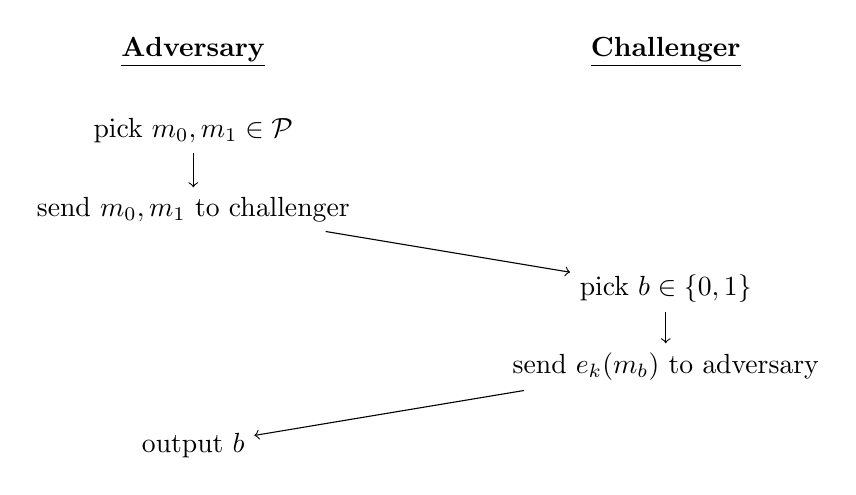
\begin{tikzpicture}
\node[] at (2, 49) {\underline{\textbf{Adversary}}};
\node[] at (8, 49) {\underline{\textbf{Challenger}}};
\node[](3) at (2, 48) {pick $m_0, m_1 \in \mathcal{P}$};
\node[](4) at (2, 47) {send $m_0, m_1$ to challenger};
\node[](5) at (8, 46) {pick $b \in \{0,1\}$};
\node[](6) at (8, 45) {send $e_k(m_b)$ to adversary};
\node[](7) at (2, 44) {output $b$};
\draw[->] (3) -- (4);
\draw[->] (4) -- (5);
\draw[->] (5) -- (6);
\draw[->] (6) -- (7);
\end{tikzpicture}

\paragraph{}
We define two kinds of security: ciphertext indistinguishability under chosen plaintext attack (IND-CPA) and ciphertext indistinguishability under chosen ciphertext attack (IND-CCA). Both have to do with how well an adversary guesses the correct $b$ in the game illustrated above, but differ what information the adversary is allowed to access in the process of playing the game.

\paragraph{}
Suppose the encryption functions are of the form $e_k: \mathcal{P} \times A \rightarrow \mathcal{C}$, where $A$ is the set over which some values are picked uniformly and randomly during encryption. Let $\mathcal{X}_{m_0, m_1}$ (resp. $\mathcal{Y}_{m_0, m_1}$) be the set of possible information available to the adversary who picked $m_0, m_1$ in the above game, in the case where the challenger chooses $b = 0$ (resp. $b = 1$).
\begin{align*}
\mathcal{X}_{m_0, m_1} &= \{ (m_0, m_1, e_k(m_0, a)) : a \in A \}\\
\mathcal{Y}_{m_0, m_1} &= \{ (m_0, m_1, e_k(m_1, a)) : a \in A \}\\
\end{align*}

\paragraph{}
Define two oracles:
\begin{itemize}
    \item $\mathcal{O}_k^\mathcal{E}$ is an encryption oracle that takes as input a plaintext $m \in \mathcal{P}$ and outputs a ciphertext $e_k(m, \dots)$, making uniform and random choices (the $\dots$ part) if required by the encryption algorithm
    \item $\mathcal{O}_k^\mathcal{D}$ is a decryption oracle that takes as input a ciphertext $c \in \mathcal{C}$ and outputs a plaintext $d_k(c)$
\end{itemize}

\paragraph{}
With these definitions in place, we can proceed to define IND-CPA and IND-CCA.

\theoremstyle{definition}
\begin{definition}{\textbf{IND-CPA}}
Let $\mathcal{A}$ be a probabilistic polynomial time adversary with access to $\mathcal{O}_k^\mathcal{E}$ who picked $m_0, m_1 \in \mathcal{P}$ in the game illustrated above. Let $X \sim \mathcal{U}(\mathcal{X}_{m_0, m_1})$ and $Y \sim \mathcal{U}(\mathcal{Y}_{m_0, m_1})$ be random variables. Then:
\begin{align*}
Adv^\mathcal{A}(X, Y) \in O(2^{-\lambda})
\end{align*}
\end{definition}

\theoremstyle{definition}
\begin{definition}{\textbf{IND-CCA}}
Let $\mathcal{A}$ be a probabilistic polynomial time adversary with access to $\mathcal{O}_k^\mathcal{D}$ who picked $m_0, m_1 \in \mathcal{P}$ in the game illustrated above. Let $X \sim \mathcal{U}(\mathcal{X}_{m_0, m_1})$ and $Y \sim \mathcal{U}(\mathcal{Y}_{m_0, m_1})$ be random variables. Then, provided the adversary does not query the oracle with the ciphertext sent by the challenger:
\begin{align*}
Adv^\mathcal{A}(X, Y) \in O(2^{-\lambda})
\end{align*}
\end{definition}

\paragraph{}
IND-CPA is equivalent to the notion of \textit{semantic security} and the two terms are often used interchangeably. In the definition of IND-CCA, if the adversary is allowed to adaptively choose ciphertexts to decrypt, it is called IND-CCA2; otherwise it is called IND-CCA1.

\subsection{Key Exchange Mechanisms}

\begin{definition}{\textbf{Key Exchange Mechanism}}
A key exchange mechanism is defined as a tuple $(\mathcal{P}, \mathcal{C}, \mathcal{K}, \overline{\mathcal{E}}, \overline{\mathcal{D}})$, where:
\begin{itemize}
    \item $\mathcal{P}$ is the set of possible plaintexts.
    \item $\mathcal{C}$ is the set of possible ciphertexts.
    \item $\mathcal{K}$ is the set of possible keys, each of which has a private component and a public component.
    \item $\overline{\mathcal{E}}$ is an \textit{encapsulation algorithm} that takes as input a public key, makes random choices (like the encryption algorithm in a public key cryptosystem) and outputs a pair $(C, K) \in \mathcal{C} \times \mathcal{P}$
    \item $\overline{\mathcal{D}}$ is a \textit{decapsulation algorithm} that takes as input both a private key and a ciphertext, and either outputs a plaintext or gives an error
\end{itemize}
\end{definition}

\paragraph{}
Following the definition in Subsection 2.2 of \cite{aggarwal2018new}, we call a key exchange mechanism $(1 - \delta)$-correct if, given a public key $k_{pub}$ and a corresponding private key $k_{pri}$, $\Pr[\overline{\mathcal{D}}(k_{pri}, C) = K | \overline{\mathcal{E}}(k_{pub}) = (C, K)] \geq 1 - \delta$.

\paragraph{}
We can give definitions of IND-CPA and IND-CCA for key exchange mechanisms as well following that given in \cite{aggarwal2018new}, with $\mathcal{O}_k^{\overline{\mathcal{E}}}$ and $\mathcal{O}_k^{\overline{\mathcal{D}}}$ being the encapsulation and decapsulation oracles respectively. Consider a fixed key $k \in \mathcal{K}$, which has a public component $k_{pub}$ and private component $k_{pri}$.

\theoremstyle{definition}
\begin{definition}{\textbf{IND-CPA}}
Let $\mathcal{A}$ be a probabilistic polynomial time adversary with access to $\mathcal{O}_k^{\overline{\mathcal{E}}}$. Let $X = (C, K_0) \sim \overline{\mathcal{E}}(k_{pub})$ and $Y = (C, K_1)$ where $K_1$ is uniformly and randomly sampled from $\mathcal{P}$. Then $Adv^\mathcal{A}(X, Y) \in O(2^{-\lambda})$.
\end{definition}

\theoremstyle{definition}
\begin{definition}{\textbf{IND-CCA}}
Let $\mathcal{A}$ be a probabilistic polynomial time adversary with access to $\mathcal{O}_k^{\overline{\mathcal{D}}}$. Let $X = (C, K_0) \sim \overline{\mathcal{E}}(k_{pub})$ and $Y = (C, K_1)$ where $K_1$ is uniformly and randomly sampled from $\mathcal{P}$. Then $Adv^\mathcal{A}(X, Y) \in O(2^{-\lambda})$, provided the adversary is not allowed to query the oracle with $C$.
\end{definition}

\section{Miscellaneous}

\theoremstyle{definition}
\begin{definition}{\textbf{Projection}}
Let $A$ be a set, $I$ be an indexing set and $B = A^{|I|}$. Then for all $i \in I$ let $\pi_i$ denote the projection onto the $i$th coordinate. That is, for all $b = \{a_j\}_{j \in I} \in B$, we have $\pi_i(b) = a_i$.
\end{definition}

\theoremstyle{definition}
\begin{definition}{\textbf{Randomness Extractor}}
Let $A$ and $B$ be sets. A randomness extractor (or extractor) is a function $Ext: A \rightarrow B$ such that $Ext(a)$ is indistinguishable from a uniformly and randomly chosen $b \in B$ for an adversary that does not know $a \in A$.
\end{definition}

\chapter{Message Extraction}\label{correctness_chapter}
\section{Overview}
\paragraph{}
In Section \ref{mersennekem_intro}, we introduced MersennePKC but did not provide an algorithm for Bob to obtain the plaintext $(A, B) \in \ham_h^n \times \ham_h^n$ given $D = AF + BG$ obtained from multiplying his private key $G$ with the ciphertext $C = A \frac{F}{G}$ sent by Alice. In this chapter, we deduce an algorithm to obtain $(A, B)$ from $D$ by way of an experiment.

\paragraph{}
We make and experimentally confirm two hypotheses:
\begin{itemize}
    \item First Iteration Hypothesis
    \item Second Iteration Hypothesis
\end{itemize}
\paragraph{}
We then use the two hypotheses to deduce an algorithm for computing $(A, B)$ from $D$.

\section{Experimental Strategy}
\paragraph{}
For the entire experiment, we fix cryptosystem parameters $n = 86243$ (a Mersenne prime) and $h = 128$. These parameters were chosen because we desire to have $h = 128$ bits of security, and $n = 86243$ is the smallest Mersenne exponent for which we obtain viable experimental results (for this value of $h$) in Section \ref{expt_results}.

\subsection{Setup} \label{correctness_strategy_setup}
\paragraph{}
The experiment is to be repeated some $N \in \N$ times.
\paragraph{}
For each repetition $\iota$ of the experiment, simulate Alice generating a random plaintext $(A, B) \in \ham_h^n \times \ham_h^n$ by sampling:
\begin{itemize}
    \item $a_1, \dots, a_h$ from $\mathcal{U}(\Z_n)$ without replacement, where $\mu(A) = \sum_{k=1}^h 2^{a_k}$
    \item $b_1, \dots, b_h$ from $\mathcal{U}(\Z_n)$ without replacement, where $\mu(B) = \sum_{k=1}^h 2^{b_k}$
\end{itemize}

\paragraph{}
We also generate Bob's private key $(F, G) \in \ham_h^n \times \ham_h^n$ in the same way, that is by sampling:
\begin{itemize}
    \item $f_1, \dots, f_h$ from $\mathcal{U}(\Z_n)$ without replacement, where $\mu(F) = \sum_{k=1}^h 2^{a_k}$
    \item $g_1, \dots, g_h$ from $\mathcal{U}(\Z_n)$ without replacement, where $\mu(B) = \sum_{k=1}^h 2^{b_k}$
\end{itemize}

\paragraph{}
Let $\alpha_\iota = \{a_1, \dots, a_h\}$. Let $D = AF + BG$.

\paragraph{}
For any subset $U \in \alpha_\iota$ we then define the following functions $\phi_\iota, \phi_{\iota, U}: \Z_n \rightarrow \Z$ in the following way:
\begin{align*}
    \phi_\iota(i) &= Ham(D) - Ham(D - 2^i F)\\
    \phi_{\iota, U}(i) &= Ham(D - \sum_{k \in U} 2^k F) - Ham(D - \sum_{k \in U} 2^k F - 2^i F)
\end{align*}

\subsection{First Iteration: Measurements and Hypothesis}

\paragraph{}
For each repetition $\iota \in \{1, \dots, N\}$, we compute
\begin{align*}
    \mathcal{I}_\iota &= \{(i, \phi_\iota(i) : i \in \alpha_\iota\}\\
    \mathcal{J}_\iota &= \{(i, \phi_\iota(i) : i \not\in \alpha_\iota\}
\end{align*}

\paragraph{}
We then compute the set of all "wanted" points $\mathcal{I}$ and the corresponding frequency map (number of occurrences of each Hamming weight) $\freq{\mathcal{I}}$:
\begin{align*}
    \mathcal{I} &= \bigcup_{\iota = 1}^N \mathcal{I}_\iota\\
    \freq{\mathcal{I}} &= \{ (m, \Delta) : m = |\{ (i, d) \in \mathcal{I} : d = \Delta \}| \}
\end{align*}

\paragraph{}
Additionally, we compute the set of points which are "unwanted", but result in the largest Hamming weight decreases (among all the unwanted points in the same repetition) when chosen. This set $\mathcal{J}_*$, together with corresponding frequency map $\freq{\mathcal{J}_*}$ is given by:
\begin{align*}
    \mathcal{J}_* &= \bigcup_{\iota = 1}^N \{ (i, d) : d = \max \pi_2(\mathcal{J}_\iota) \}\\
    \freq{\mathcal{J}_*} &= \{ (m, \Delta) : m = |\{ (i, d) \in \mathcal{J}_* : d = \Delta \}| \}
\end{align*}

\paragraph{}
We then plot two histograms: $H_\mathcal{I}$ for $\freq{\mathcal{I}}$ and $H_{\mathcal{J}_*}$ for $\freq{\mathcal{J}_*}$ . We fit the normal distributions $N(\mu_\mathcal{I}, \sigma_\mathcal{I}^2)$ and $N(\mu_{\mathcal{J}_*}, \sigma_{\mathcal{J}_*}^2)$ onto $H_\mathcal{I}$ and $H_{\mathcal{J}_*}$ respectively.

\paragraph{\textbf{First Iteration Hypothesis}} Let $X \sim N(\mu_{\mathcal{J}_*}, \sigma_{\mathcal{J}_*}^2)$. We hypothesise that the respective means and variances take on values such that $Pr[X \geq \mu_\mathcal{I}] \approx 10^{-29}$.

\paragraph{}
For each repetition $\iota$, we choose a set of points $U_\iota$ by skimming off all the indices that yield Hamming weight reductions more than $\mu_\mathcal{I}$:
\begin{align*}
    U_\iota = \{ i \in \Z_n : \phi_\iota(i) > \mu_\mathcal{I} \}
\end{align*}

\paragraph{}
Assuming the first iteration hypothesis, $U_\iota \subseteq \alpha_\iota$ with high probability, for each repetition $\iota$.

\subsection{Second Iteration: Measurements and Hypothesis}
\paragraph{}
We then compute:
\begin{align*}
    \mathcal{I}_\iota' &= \{(i, \phi_{\iota, U}(i) : i \in \alpha_\iota \backslash U_\iota\}\\
    \mathcal{J}_\iota' &= \{(i, \phi_{\iota, U}(i) : i \not\in \alpha_\iota \backslash U_\iota\}
\end{align*}

\paragraph{}
We repeat all the calculations as in the first iteration, replacing $\mathcal{I}_\iota$ and $\mathcal{J}_\iota$ by $\mathcal{I}_\iota'$ and $\mathcal{J}_\iota'$ respectively:
\begin{align*}
    \mathcal{I}' &= \bigcup_{\iota = 1}^N \mathcal{I}_\iota'\\
    \freq{\mathcal{I}'} &= \{ (m, \Delta) : m = |\{ (i, d) \in \mathcal{I}' : d = \Delta \}| \}\\
    \mathcal{J}_*' &= \bigcup_{\iota = 1}^N \{ (i, d) : d = \max \pi_2(\mathcal{J}_\iota') \}\\
    \freq{\mathcal{J}_*'} &= \{ (m, \Delta) : m = |\{ (i, d) \in \mathcal{J}_*' : d = \Delta \}| \}
\end{align*}

\paragraph{}
We then plot two new histograms: $H_{\mathcal{I}'}$ for $\freq{\mathcal{I}'}$ and $H_{\mathcal{J}_*'}$ for $\freq{\mathcal{J}_*'}$ . We fit the normal distributions $N(\mu_{\mathcal{I}'}, \sigma_{\mathcal{I}'}^2)$ and $N(\mu_{\mathcal{J}_*'}, \sigma_{\mathcal{J}_*'}^2)$ onto $H_{\mathcal{I}'}$ and $H_{\mathcal{J}_*'}$ respectively.

\paragraph{\textbf{Second Iteration Hypothesis}} Let $Y \sim N(\mu_{\mathcal{J}_*'}, \sigma_{\mathcal{J}_*'}^2)$. We hypothesise that the respective means and variances take on values such that $Pr[Y \geq \mu_{\mathcal{I}'} - 4 \sigma_{\mathcal{I}'}] \approx 10^{-28}$.

\paragraph{}
For each repetition $\iota$, we choose a set of points $U_\iota'$ by skimming off all the indices that yield Hamming weight reductions more than $\mu_{\mathcal{I}'} - 4 \sigma_{\mathcal{I}'}$:
\begin{align*}
    U_\iota' = \{ i \in \Z_n : \phi_{\iota, U_\iota}(i) > \mu_{\mathcal{I}'} - 4 \sigma_{\mathcal{I}'} \}
\end{align*}

\paragraph{}
Assuming the second iteration hypothesis, $U_\iota' \subseteq \alpha_\iota$ with high probability, for each repetition $\iota$.

\section{Experimental Results}\label{expt_results}

\subsection{First Iteration}
\paragraph{}
We plot the histograms $H_{\mathcal{I}}$ (green portion) and $H_{\mathcal{J}_*}$ (red portion) for the first iteration. The data for $H_{\mathcal{I}}$ has a sample mean of $74.5$ and sample variance of $8.64^2$. The data for $H_{\mathcal{J}_*}$ has a sample mean of $25.9$ and sample variance of $4.17^2$.
\paragraph{}
We fit normal distributions to both histograms by method of moments estimation and obtain:
\begin{align*}
    \mu_\mathcal{I} &= 74.5\\
    \sigma_\mathcal{I} &= 8.64\\
    \mu_{\mathcal{J}_*} &= 25.9\\
    \sigma_{\mathcal{J}_*} &= 4.17
\end{align*}

Letting $X \sim N(\mu_{\mathcal{J}_*}, \sigma_{\mathcal{J}_*}^2)$ we use the Gaussian tail bound to obtain:
\begin{align*}
    Pr[X \geq \mu_\mathcal{I}] &= Pr[X - \mu_{\mathcal{J}_*} \geq \mu_\mathcal{I} - \mu_{\mathcal{J}_*}]\\
    &= Pr[X - \mu_{\mathcal{J}_*} \geq 74.5 - 25.9]\\
    &= Pr[X - \mu_{\mathcal{J}_*} \geq 48.6]\\
    &\leq \exp{(-\frac{48.6^2}{2 \sigma_{\mathcal{J}_*}^2})}\\
    &= \exp{(-\frac{48.6^2}{2 \times 4.17^2})}\\
    &\leq 3.20 \times 10^{-30}
\end{align*}

\paragraph{}
This confirms the first iteration hypothesis.

\paragraph{}
\includegraphics[scale=0.75]{mersennepkc_extraction_first.png}\newline

\subsection{Second Iteration}
\paragraph{}
We plot the histograms $H_{\mathcal{I}'}$ (green portion) and $H_{\mathcal{J}_*'}$ (red portion) for the first iteration. The data for $H_{\mathcal{I}'}$ has a sample mean of $87.5$ and sample variance of $6.65^2$. The data for $H_{\mathcal{J}_*'}$ has a sample mean of $11.9$ and sample variance of $4.35^2$.
\paragraph{}
We fit normal distributions to both histograms by method of moments estimation and obtain:
\begin{align*}
    \mu_{\mathcal{I}'} &= 87.5\\
    \sigma_{\mathcal{I}'} &= 6.65\\
    \mu_{\mathcal{J}_*'} &= 11.9\\
    \sigma_{\mathcal{J}_*'} &= 4.35
\end{align*}

Letting $Y \sim N(\mu_{\mathcal{J}_*'}, \sigma_{\mathcal{J}_*'}^2)$ we use the Gaussian tail bound to obtain:
\begin{align*}
    Pr[Y \geq \mu_{\mathcal{I}'} - 4 \sigma_{\mathcal{I}'}] &= Pr[Y - \mu_{\mathcal{J}_*'} \geq \mu_{\mathcal{I}'} - 4 \sigma_{\mathcal{I}'} - \mu_{\mathcal{J}_*'}]\\
    &= Pr[Y - \mu_{\mathcal{J}_*'} \geq 87.5 - 4 \times 6.65 - 11.9]\\
    &= Pr[Y - \mu_{\mathcal{J}_*'} \geq 49.0]\\
    &\leq \exp{(-\frac{49.0^2}{2 \sigma_{\mathcal{J}_*'}^2})}\\
    &= \exp{(-\frac{49.0^2}{2 \times 4.35^2})}\\
    &\leq 2.80 \times 10^{-28}
\end{align*}

\paragraph{}
This confirms the second iteration hypothesis.

\includegraphics[scale=0.75]{mersennepkc_extraction_second.png}

\section{Deducing the Algorithm}\label{msg_ext_deduction}

At this point, we have experimentally verified the two hypotheses we made earlier. We can now use these hypotheses to obtain an algorithm $\chi_{n, h}$ to extract $(A, B)$ given $D$:
\begin{align*}
\chi_{n, h} &: \mathcal{B}_n \times \ham_h^n \times \ham_h^n \rightarrow \ham_h^n \times \ham_h^n\\
\chi_{n, h} &= (AF + BG, F, G) \mapsto (A, B)
\end{align*}

\subsection{Proposed Algorithm}\label{proposed_algo}
\paragraph{}
Suppose it is known that $A, B, F, G \in \ham_h^n$, where $F$ and $G$ is known to Bob while $A$ and $B$ is not. Suppose Bob has $D = AF + BG \in \mathcal{B}_n$ and wishes to compute $(A, B) \in \ham_h^n \times \ham_h^n$. We propose an procedure EXTRACT-MSG to do so:

\begin{lstlisting}[mathescape=true]
EXTRACT-MSG(n, h, D, F, G):
    A := 0
    B := 0
    
    for k in {0, 1}
        maintain a loop counter $k$
        
        for i: $\Z_n$ in {0, .., n-1}:
            if HAMMING-WEIGHT-DECREASE(D, F, i) >= $\delta_k$:
                set bit i of A
            if HAMMING-WEIGHT-DECREASE(D, G, i) >= $\delta_k$:
                set bit i of B
        
        D := D - (A * F + B * G)
    
    if Ham(A) != h or Ham(B) != h:
        error
    
    return (A, B)
\end{lstlisting}
\newpage

\paragraph{}
The procedure EXTRACT-MSG depends on a threshold $\delta_k$ for $k \in \{0, 1\}$. From the experimental results used to confirm the iteration hypotheses, we set:
\begin{align*}
    \delta_0 &= \mu_{\mathcal{I}}\\
    &= 74.5\\
    \delta_1 &= \mu_{\mathcal{I}'} - 4 \sigma_{\mathcal{I}'}\\
    &= 87.5 - 4 \times 6.65\\
    &= 60.9
\end{align*}

\paragraph{}
The procedure EXTRACT-MSG also depends on a subprocedure:

\begin{lstlisting}
HAMMING-WEIGHT-DECREASE(D, X, i):
    return HAM(D) - HAM(D - X * 2^i)
\end{lstlisting}

\subsection{Probabilistic Correctness of Algorithm}
\paragraph{}
The algorithm has two main iterations, with the main body of each iteration taking place in lines 6-14. We analyse what happens in those two iterations, as well as the error check that takes place in lines 16-17.

\paragraph{}
Let $\alpha$ and $\beta$ be the (unknown) sets, both of size $h$, such that:
\begin{align*}
    A &= \sum_{i \in \alpha} 2^i\\
    B &= \sum_{j \in \beta} 2^j
\end{align*}
To avoid unwieldy prose in the paragraphs that follow, we define the Hamming weight decrease function (the same one as in HAMMING-WEIGHT-DECREASED) by:
\begin{align*}
    \phi &: \mathcal{B}_n \times \ham_h^n \times \Z_n \rightarrow \Z\\
    \phi &= (D, X, i) \mapsto Ham(D) - Ham(D - X * 2^i)
\end{align*}

\paragraph{Probability of Wrong Index Being Chosen}
We first analyse the probability that the algorithm chooses a wrong index to set in either $A$ or $B$. This wrong choice can happen in either of the two iterations of the loop in Line 5.

\paragraph{}
Let $\alpha_0, \beta_0 \subseteq \Z_n$ be the indices chosen and set in the first iteration for $A$ and $B$ respectively. Let $E_{A,0}$ and $E_{B,0}$ be the events that $\alpha_0 \subseteq \alpha$ and $\beta_0 \subseteq \beta$ respectively. By the first iteration hypothesis, we have:
\begin{align*}
    Pr[\overline{E_{A,0}}] &\approx 10^{-29}\\
    Pr[\overline{E_{B,0}}] &\approx 10^{-29}
\end{align*}

\paragraph{}
Let $\alpha_1, \beta_1$ be the indices chosen and set in the second iteration for $A$ and $B$ respectively. Let $E_{A,1}$ and $E_{B,1}$ be the events that $\alpha_1 \subseteq \alpha \backslash \alpha_0$ and $\beta_1 \subseteq \beta \backslash \beta_0$ respectively. By the second iteration hypothesis, we have:
\begin{align*}
    Pr[\overline{E_{A,1}} | \overline{E_{A,0}}] &\approx 10^{-28}\\
    Pr[\overline{E_{B,1}} | \overline{E_{A,0}}] &\approx 10^{-28}
\end{align*}

\paragraph{}
Let $E_A$ and $_B$ be the events that a wrong index is chosen for $A$ and $B$ respectively. We have:
\begin{align*}
    Pr[E_A] &= Pr[E_{A,0}] + Pr[\overline{E_{A,0}}] \times Pr[E_{A,1} | \overline{E_{A,0}}]\\
    &\approx 10^{-29} + (1 - 10^{-29}) \times 10^{-28}\\
    &\approx 10^{-28}\\
    Pr[E_B] &= Pr[E_{B,0}] + Pr[\overline{E_{B,0}}] \times Pr[E_{B,1} | \overline{E_{B,0}}]\\
    &\approx 10^{-28} \text{     (by similar reasoning)}
\end{align*}

\paragraph{}
Let $E$ be the event that the algorithm chooses the wrong index at any time. Then $Pr[E] \leq Pr[E_A] + Pr[E_B] < 2 \times 10^{-28}$. We have therefore established that the algorithm picks the wrong index with extremely low probability. \qed

\paragraph{\textbf{Probability of Insufficient Number of Indices being Chosen}}
Assuming that no incorrect point has been selected, we note that the error condition in line 16 triggers when $\alpha_0 \cup \alpha_1 \not= \alpha$, that is, when there are indices that remain unselected.

\paragraph{}
Let $E'$ be the probability that at least one point that should have been selected but was not. Let $Z \sim N(\mu_{\mathcal{I}'}, \sigma_{\mathcal{I}'}^2)$. Then we have:
\begin{align*}
    Pr[E' | \overline{E}] &= Pr[Z < \mu_{\mathcal{I}'} - 4 \sigma_{\mathcal{I}'}]\\
    &= Pr[\frac{Z - \mu_{\mathcal{I}'}}{\sigma_{\mathcal{I}'}} < -4]\\
    &= \int_{-\infty}^{-4} \frac{1}{\sqrt{2 \pi}} \exp{(-\frac{x^2}{4})} dx\\
    &< 1.34 \times 10^{-4}
\end{align*}

\paragraph{}
We therefore have that the probability of an insufficient number of points is somewhat high (order of $10^{-4}$) compared to the probability of error. This, however, is not a cause for concern since we can simply repeat the loop in line 5 as many times as needed in the rare that an insufficient number of points are selected. \qed

\paragraph{}
We have seen that the message extraction algorithm presented in this section computes the correct $(A,B)$ from $D$ with very high probability (with a small, non-negligible but acceptable chance of needing to run for more than two iterations). We now turn to the runtime of the algorithm.

\subsection{Runtime Of Algorithm}
\paragraph{}
In Subsection \ref{proposed_algo}, we gave an implementation of EXTRACT-MSG and HAMMING-WEIGHT-DECREASE. We first give the time complexity of EXTRACT-MSG in terms of the time complexity of HAMMING-WEIGHT-DECREASE, which we call $T(n)$.

\begin{lemma}
EXTRACT-MSG runs in time $O(n T(n) + nh)$.
\end{lemma}
\paragraph{\textbf{Proof}}
We see that lines 8-14 runs in $O(n T(n))$, since setting bits is $O(1)$ and the loop body (which takes $O(T(n) + 1) = O(T(n))$ is run $n$ times in the loop defined on line 8. Line 14 has multiplications $A*F$ and $B*G$ that take $O(nh)$ since $F$ and $G$ have Hamming weight $h$ and we can simply perform $A*F = \sum_{k = 1}^h A \times 2^{f_k}$ and $B*G = \sum_{k = 1}^h B \times 2^{g_k}$ where $f_1, \dots f_h$ are the bits set in $F$ and $g_1, \dots, g_h$ are the bits set in $G$.

\paragraph{}
The body of the loop in line 5 therefore runs in $O(nT(n) + nh)$, so the entire loop (which makes only a constant number of iterations) runs in $O(nT(n) + nh)$. The check on lines 16-17 run in $O(n)$ since they perform a Hamming weight computation, while the initialisation code on lines 2-3 take $O(n)$ as they allocate memory for bitstrings of length $n$.

\paragraph{}
We can therefore conclude that EXTRACT-MSG runs in $O(nT(n) + nh)$. \qed

\paragraph{}
We note that, from our current implementation, HAMMING-WEIGHT-DECREASE runs in time $O(n)$. This is because all the steps (Hamming weight computation, subtraction, bit shifting) are all linear in the number of bits operated on, which is $n$. This makes the time complexity of EXTRACT-MSG $O(n^2 + nh) = O(n^2)$ since $n > 2 h^2$. With $n = 86243$, the number of operations to be performed is on the order of $10^9$, which is rather large. We therefore propose a functionally-equivalent but more efficient implementation of HAMMING-WEIGHT-DECREASE.

\begin{lstlisting}[mathescape=true]
HAMMING-WEIGHT-DECREASE'(D, X, i):
    compute Y := X * $2^i$
    
    // ensure D > Y, this makes the result off by at most 1
    pad D with an additional bit on the MSB side
    
    //can view D as a bit sequence $d_r \dots d_1$
    //can view Y as an ordered set of indices $\{ y_{j_1}, \dots, y_{j_h} \}$
    
    ham_wt_reduction := 0
    stop := set bit in D with smallest index greater than $y_{j_h}$
    
    for k from h downto 1:
        if $y_{j_k}$ = 0:
            if $d_{j_k}$ = 1:
                stop := $j_k$
            continue
        ham_wt_reduction -= 1
        if $d_{j_k}$ = 1:
            $d_{j_k}$ := 0
        else:
            c := stop - i
            ham_wt_reduction += c
            stop = i
    return ham_wt_reduction
        
\end{lstlisting}

\paragraph{}
The idea behind HAMMING-WEIGHT-DECREASE' is to count the number of places where the Hamming weight could change during subtraction, rather than actually performing the subtraction.
\begin{itemize}
    \item If both the minuend and subtrahend have a bit set at a given index, then the Hamming weight is guaranteed to decrease by exactly one at that index.
    \begin{itemize}
        \item e.g. $110$ - $010$ causes a Hamming weight decrease of one at index $2$
        \item e.g. $11011$ - $1000$ causes a Hamming weight decrease of one at index $4$
    \end{itemize}
    \item If the subtrahend has a bit set at the index but the minuend does not, then the Hamming weight is guaranteed to increase by one less than the number of zeros in the minuend starting from that index and counting upward until the next set bit.
    \begin{itemize}
        \item e.g $10000 - 1$ will cause a Hamming weight increase of $4 - 1 = 3$ since the result becomes $01111$
        \item e.g. $10000 - 10$ will cause a Hamming weight increase of $3 - 1 = 2$ since the result becomes $01110$
    \end{itemize}
\end{itemize}

\paragraph{}
The algorithm searches (the loop in Line 13) all the indices of bits set in the subtrahend (at most $h$ many) and keeps track of the Hamming weight changes when each particular bit of the subtrahend is subtracted from the minuend. When the algorithm terminates, it will return the total Hamming weight change when the entire subtrahend has been subtracted from the minuend, which is what we want.

\begin{claim}
HAMMING-WEIGHT-DECREASE' runs in $O(h)$.
\end{claim}
\begin{proof}
Line 2 runs in $O(h)$ since $X$ has Hamming weight $h$.
Lines 5 and 10 can be done in $O(1)$.
Line 11 can be done in $O(1)$ on average by starting at $d_{j_h}$ and searching upwards, since $D$ is expected to be somewhat dense and no more than a very small number of positions are searched on average.
Every step in Lines 14-24 takes $O(1)$, so the entire loop from Lines 13-24 takes $O(h)$.
\end{proof}

\paragraph{}
Therefore, using HAMMING-WEIGHT-DECREASE' in place of HAMMING-WEIGHT-DECREASE, EXTRACT-MSG has time complexity $O(nh)$. With $n = 86243, h = 128$, this is of order $10^6$, which is very fast on a modern computer.

\paragraph{}
Having obtained an efficient algorithm to compute $(A,B)$ given $D$, we now turn to constructing the key-exchange protocol in the following chapter.

\chapter{Public Key Cryptosystem}\label{description_chapter}
\section{Overview}
\paragraph{}
Before we give a formal specification of MersennePKC, we first give an illustration of how it is expected to work intuitively.

\paragraph{}
Let $n, h \in \N$ such that $n > 2h^2$ and $2^n - 1$ is a Mersenne prime. Suppose we have an extractor $Ext: \ham_h^n \times \ham_h^n \rightarrow \F_2^\lambda$, for some $\lambda \in \N$.

\paragraph{}
We assume that we have two agents Alice and Bob. Suppose Bob has private key $(F, G) \in \ham_h^n \times \ham_h^n$ and public key $H = \frac{F}{G} \in \mathcal{B}_n$. Then an Alice can send a message $m \in \F_2^\lambda$ to Bob via the following protocol:

\begin{tikzpicture}
\node[] at (2, 50) {\underline{\textbf{Alice}}};
\node[] at (8, 50) {\underline{\textbf{Bob}}};
\node[](1) at (2, 49) {$A, B \sim \mathcal{U}(\ham_h^n)$};
\node[](2) at (2, 48) {$C := A H + B$};
\node[](3) at (2, 47) {$c := Ext(A, B) \oplus m$};
\node[](4) at (2, 46) {send $(C, c)$ to Bob};
\node[](5) at (8, 46) {receive $(C, c)$ from Alice};
\draw[->] (4) -- (5);
\node[](6) at (8, 45) {$D := CG$};
\node[](7) at (8, 44) {$(A,B) := \chi_{n, h}(D, F, G)$};
\node[](8) at (8, 43) {$m := Ext(A, B) \oplus c$};
\draw (-1, 42) rectangle (11, 51);
\end{tikzpicture}

\paragraph{}
In the protocol above, Alice first uniformly and randomly samples $A$ and $B$ from $\ham_h^n$. She then sends the pair $(C, c) = (AH + B, Ext(A, B) \oplus m)$ over an insecure channel to Bob, where $H$ is Bob's public key.

\paragraph{}
Bob receives $(C, c)$ from Alice and computes $D = CG$ using the $G$ component of his private key. He then uses the message extraction algorithm described in Chapter \ref{correctness_chapter} to recover $A$ and $B$ from $D$. He finally computes $Ext(A,B) \oplus c = Ext(A, B) \oplus Ext(A, B) \oplus m = m$, thereby retrieving the plaintext.

\paragraph{}
Having illustrated the functioning of MersennePKC, we proceed to its formal specification.

\section{Specification}
\theoremstyle{definition}
\begin{definition}{\textbf{MersennePKC}}\label{mersennepkc-specification}
Let $n, h \in \N$ be fixed parameters such that $n \geq 2h^2$ and $p = 2^n -1$ is a Mersenne prime. Let $Ext: \ham_h^n \times \ham_h^n \rightarrow \F_2^\lambda$ be an extractor. MersennePKC-($n, h, Ext$) is the tuple $(\mathcal{P}, \mathcal{C}, \mathcal{K}, \mathcal{E}, \mathcal{D})$ where:
\begin{align*}
    \mathcal{P} =\:&\F_2^\lambda\\
    \mathcal{C} =\:&\mathcal{B}_n \times \F_2^\lambda\\
    \mathcal{K} =\:&\{ (F, G, H) \in \ham_h^n \times \ham_h^n \times \mathcal{B}_n : H = \frac{F}{G} \}\\
    \mathcal{E} =\:&\{e_k: \ham_h^n \times \ham_h^n \times \mathcal{P} \rightarrow \mathcal{C} :\\
    &\:k = (F, G, H) \in \mathcal{K},\\
    &\:e_k(A, B, m) = (AH + B, Ext(A, B) \oplus m) \}\\
    \mathcal{D} =\:&\{ d_k: \mathcal{C} \rightarrow \mathcal{P} :\\
    &\:k = (F, G, H) \in \mathcal{K},\\
    &\:d_k(C, c) = Ext(\chi_{n, h}(CG, F, G)) \oplus c \}
\end{align*}
\end{definition}

\paragraph{}
In the definition above, the cryptosystem explicitly depends on the choices of $n$, $h$ and the extractor $Ext$, and also implicitly depends on $\lambda$ via $Ext$.
\begin{itemize}
    \item $\mathcal{P}$ is the set of plaintexts.
    \item $\mathcal{C}$ is the set of ciphertexts.
    \item $\mathcal{K}$ is the set of keys. Each key has the form $(F, G, H)$, where $(F, G)$ is the private key while $H$ is the public key.
    \item $\mathcal{E}$ is the set of encryption functions. Each encryption function $e_k$ depends on a key $k$, and is of the form $\ham_h^n \times \ham_h^n \times \mathcal{P} \rightarrow \mathcal{C}$. The extra input from $\ham_h^n \times \ham_h^n$ in addition to the plaintext is meant for the encryptor to supply uniform random choices to allow for semantic security.
    \item $\mathcal{D}$ is the set of decryption functions. Each decryption function $d_k$ depends on a key $k$, and uses $\chi_{h_h}$ from Chapter \ref{correctness_chapter} as part of its decryption.
\end{itemize}

\section{Security}

\paragraph{}
We can see from the illustration of MersennePKC that any adversary intercepting the insecure communications channel between Alice and Bob is able to obtain the following information:
\begin{itemize}
    \item cryptosystem parameters $n, h$, known publicly
    \item Bob's public key, $H$, known publicly
    \item ciphertext $(C, c)$ that Alice sends to Bob over the channel during the key exchange
\end{itemize}

\paragraph{}
We want to see how secure MersennePKC is under chosen plaintext attacks (IND-CPA) and chosen ciphertext attacks (IND-CCA).

\paragraph{}
For the rest of this section, we assume that $(\mathcal{P}, \mathcal{C}, \mathcal{K}, \mathcal{E}, \mathcal{D})$ is a MersennePKC-($n, h, Ext$) instance, where $Ext: \ham_h^n \times \ham_h^n \rightarrow \F_2^\lambda$ is an extractor, $h$ is the security parameter and $\lambda = h$.

\paragraph{}
For each key $k = (F, G, H) \in \mathcal{K}$, we define two oracles.
\begin{itemize}
    \item Let $\mathcal{O}_k^\mathcal{E}$ be an encryption oracle that encrypts a plaintext $m \in \mathcal{P}$ to $(AH + B, Ext(A, B) \oplus m) \in \mathcal{C}$, where $A$ and $B$ are uniformly and randomly chosen from $\ham_h^n$.
    \item Let $\mathcal{O}_k^\mathcal{D}$ be a decryption oracle that decrypts a ciphertext $(C, c) \in \mathcal{C}$ to $Ext(A, B) \oplus c \in \mathcal{P}$, where $C = A \frac{F}{G} + B$.
\end{itemize}

\subsection{Chosen Plaintext Attacks}
\paragraph{}
MersennePKC is secure under chosen plaintext attacks (IND-CPA), subject to some assumptions.

\begin{assumption}\label{assumpt_pubkey_appears_uniform}
Let $\mathcal{A}$ be a probabilistic polynomial-time Turing machine. Let $(F, G, H) \in \mathcal{K}$. Define the following probability distributions:
\begin{align*}
\mathcal{X} &= \mathcal{U}(\{ AH + B: A, B \in \ham_h^n  \})\\
\mathcal{Y} &= \mathcal{U}(\mathcal{B}_n)
\end{align*}
The task of $\mathcal{A}$ is to output $0$ if its input comes from $\mathcal{X}$ and $1$ if its input comes from $\mathcal{Y}$. Let $X \sim \mathcal{X}$ and $Y \sim \mathcal{Y}$ be random variables. Then $Adv^\mathcal{A}(X, Y) \in O(2^{-h})$.
\qed
\end{assumption}

\begin{assumption}\label{assumpt_extracted_value_appears_uniform}
Let $\mathcal{A}$ be a probabilistic polynomial-time Turing machine. Define the following probability distributions:
\begin{align*}
\mathcal{X} &= \mathcal{U}(\{ Ext(A, B): A, B \in \ham_h^n  \})\\
\mathcal{Y} &= \mathcal{U}(\mathcal{B}_n)
\end{align*}
The task of $\mathcal{A}$ is to output $0$ if its input comes from $\mathcal{X}$ and $1$ if its input comes from $\mathcal{Y}$. Let $X \sim \mathcal{X}$ and $Y \sim \mathcal{Y}$ be random variables. Then $Adv^\mathcal{A}(X, Y) \in O(2^{-h})$.
\qed
\end{assumption}

\paragraph{}
Assumption \ref{assumpt_pubkey_appears_uniform} claims that the public keys appear uniformly random on $\mathcal{B}_n$ and do not leak information about the private key. Assumption \ref{assumpt_extracted_value_appears_uniform} claims that $Ext(A, B)$ does not leak any information about $AH+B$ (and therefore does not leak any information about $A$ or $B$).

\paragraph{}
With these assumptions, we can now show that MersennePKC is secure under chosen plaintext attacks.

\begin{theorem}{\textbf{MersennePKC satisfies IND-CPA}}
Fix some key $k = (F, G, H) \in \mathcal{K}$. Let $\mathcal{A}$ be a probabilistic polynomial-time adversary with access to $H$ and $\mathcal{O}_k^\mathcal{E}$ who chooses $m_0, m_1 \in \mathcal{P}$. Define the following random variables:
\begin{align*}
Z_0 &\sim \mathcal{U}(\{ (AH + B, Ext(A, B) \oplus m_0) : A, B \in \ham_h^n \})\\
Z_1 &\sim \mathcal{U}(\{ (AH + B, Ext(A, B) \oplus m_1) : A, B \in \ham_h^n \})\\
\end{align*}
Then $Adv^\mathcal{A}(Z_0, Z_1) \in O(2^{-h})$ regardless of the choice of $m_0, m_1 \in \mathcal{P}$ that $\mathcal{A}$ makes.
\end{theorem}
\begin{proof}
The goal is for $\mathcal{A}$ to output $b$ given $(C, c) = (AH + B, Ext(A, B) \oplus m_b)$. There are two ways to do this: attempting to recover information about $A$ and $B$ (and hence $Ext(A, B)$ by obtaining information about the private key $F$ and $G$, or using $AH + B$ to obtain information about $Ext(A, B)$.
\newline
By Assumption \ref{assumpt_pubkey_appears_uniform}, the public key appears uniform and random to $\mathcal{A}$. Extracting any information about the private key from the public key allows $\mathcal{A}$ to distinguish the public key from a random bitstring sampled from $\mathcal{U}(\mathcal{B}_n)$, and so the advantage of $\mathcal{A}$ in doing so is bounded above by $O(2^{-h})$.
\newline
By Assumption \ref{assumpt_extracted_value_appears_uniform}, the advantage of $\mathcal{A}$ in obtaining any information about $Ext(A, B)$ from $AH + B$ is bounded above by $O(2^{-h})$.
\newline
Since $\mathcal{A}$ needs to only succeed at one of the two attempts to distinguish $Z_0$ from $Z_1$, the probability of distinguishing them is bounded above by the sum of the probabilities of distinguishing them using each approach. Therefore, for some $\alpha, \beta \in \N$:
\begin{align*}
Adv^\mathcal{A}(Z_0, Z_1) &\in O(2^{-h}) + O(2^{-h})\\
&= O(2^{-h})
\end{align*}
\end{proof}

\subsection{Chosen Ciphertext Attacks}
\paragraph{}
MersennePKC, as given above, fails to satisfy even IND-CCA1 i.e. it is vulnerable to nonadaptive chosen ciphertext attacks.

\paragraph{}
Suppose an probabilistic polynomial-time adversary with access to $\mathcal{O}_k^\mathcal{D}$ chooses $m_0, m_1 \in \mathcal{P}$, is given $(C, c) = (AH + B, Ext(A, B) \oplus m_b) \in \mathcal{C}$ by the challenger and needs to determine $b \in \{0, 1\}$. The adversary simply queries $\mathcal{O}_k^\mathcal{D}$ with the ciphertext $(AH + B, 0^\lambda)$. The oracle gives $m' = Ext(A, B) \oplus 0^\lambda = Ext(A, B)$ to the adversary, who then computes $c \oplus m' = Ext(A, B) \oplus m_b \oplus Ext(A, B) = m_b$ and compares the result with $m_0$ and $m_1$. In this way, the adversary can determine $b$, so MersennePKC as given does not satisfy IND-CCA1.

\paragraph{}
To make MersennePKC secure under chosen ciphertext attacks, we use a technique similar to that in Section 7 of \cite{aggarwal2018new}: turning the MersennePKC-($n, h, Ext$) instance into a key encapsulation mechanism and using a random oracle to transform the randomly selected key. We call this new key encapsulation mechanism MersenneKEM-($n, h, Ext$).

\theoremstyle{definition}
\begin{definition}{\textbf{MersenneKEM}}
Suppose $\mathcal{H}_0$ and $\mathcal{H}_1$ are random oracles with input $\F_2^\lambda$ and output $\ham_h^n$.
\begin{itemize}
    \item Let $\overline{\mathcal{E}}$ be an algorithm that takes as input a public key $H$, samples $K \sim \mathcal{U}(\F_2^\lambda)$, computes $A = \mathcal{H}_0(K), B = \mathcal{H}_1(K)$ and outputs $(AH + B, Ext(A, B) \oplus K$.
    \item Let $\overline{\mathcal{D}}$ be an algorithm that as input a private key $(F, G)$ and ciphertext $(C, c)$, retrieves $(A', B')$ from $CG$ using the message extraction algorithm from Chapter \ref{correctness_chapter}, computes $K' = Ext(A', B') \oplus c$, and outputs $K'$ if $A'H + B' = C$ or gives an error otherwise. 
\end{itemize}
MersenneKEM-($n, h, Ext$) is the tuple $(\mathcal{P}, \mathcal{C}, \mathcal{K}, \overline{\mathcal{E}}, \overline{\mathcal{D}})$.
\end{definition}

\begin{theorem}{\textbf{MersenneKEM satisfies IND-CCA}}\label{mersennekem-ind-cca}
Fix some key $k = (F, G, H) \in \mathcal{K}$. Let $\mathcal{A}$ be a probabilistic polynomial-time adversary with access to $H$ and an oracle $\mathcal{O}_k^{\overline{\mathcal{D}}}$ to perform decapsulation. Let $X = (C, K_0) \sim \overline{\mathcal{E}}(F, G)$ and $Y = (C, K_1)$ where $K_1$ is uniformly and randomly sampled from $\mathcal{P}$. Then $Adv^\mathcal{A}(X, Y) \in O(2^{-h})$.
\end{theorem}

\paragraph{}
The proof of Theorem \ref{mersennekem-ind-cca} is identical to that of Theorem 2 in \cite{aggarwal2018new}, although the key exchange protocols are different.

\section{Extractors}
\paragraph{}
MersennePKC and MersenneKEM are defined with respect to an extractor function, in addition to $n$ and $h$. Since we set the security parameter $\lambda$ to $h$, we expect the extractors to have the type $Ext: \ham_h^n \times \ham_h^n \rightarrow \F_2^h$.

\paragraph{}
Since we set $h = 128$, we can generally use any cryptographic hash function that outputs a $128$-bit string as an extractor. However, in the interest of efficiency in encryption and decryption, we opt to use a simpler extractor involving the inner product. Before we take an inner product, we perform a sequence of transformations to remove any unnecessary bits not contributing to the entropy of the source strings used in the extractor.

\paragraph{}
Suppose we have $A \in \ham_h^n$, which is a bitstring that typically consists of clusters of $0$s separated by a small number of $1$s. Since $A$ has Hamming weight $h$, there are at most $h+1$ clusters. Each cluster has at most $n$ elements since the entire string $A$ has only $n$ bits. We can therefore identify the sequence of clusters with a vector in $\Z_n^{h+1}$. We define a map $f: \ham_h^n \rightarrow \Z_n^{h+1}$ to represent this identification.

\paragraph{}
We then define the map $g: \Z_n^{h+1} \rightarrow \F_2^{(h+1) \log{n}}$ in the following manner: given an input $x \in \Z_n^{h+1}$, concatenate the bit representations of all the elements in the vector without the leading one (which does not contribute to the entropy of the result) into a single bitstring $y$. Since each element of $x$ has at most $\log{n}$ bits (being an element of $\Z_n$) and $x$ has $h+1$ elements, it follows that $y \in \F_2^{(h+1) \log{n}}$.

\paragraph{}
We finally define the map $h: \F_2^{(h+1) \log{n}} \rightarrow \F_{2^h}^m$, for the appropriate choice of $m$, by regarding each element of $\F_2^{(h+1) \log{n}}$ as an element in $\F_{2^h}^m$. This $m$ will be sligtly greater than $\log{n}$, and the bitstrings in $\F_2^{(h+1) \log{n}}$ may be padded if necessary.

\theoremstyle{definition}
\begin{definition}{\textbf{Inner Product Extractor}}
Define $Ext: \ham_h^n \times \ham_h^n \rightarrow \F_{2^h}$ in the following way:
\begin{align*}
    Ext(A, B) &= <h \circ g \circ f(A), h \circ g \circ f(B)>
\end{align*}
We then identify $\F_{2^h}$ with $\F_2^h$ by identifying elements in $\F_{2^h}$ with their bit representations, and obtain an extractor $Ext: \ham_h^n \times \ham_h^n \rightarrow \F_2^h$.
\end{definition}

\paragraph{}
The inner product extractor appears uniform and random to an adversary without access to $A$ or $B$: this is a standard result from \cite{chor1988unbiased}. This extractor is not secure under information leakage; however, it may be transformed accordingly using methods from \cite{dziembowski2011leakage} if needed.

\paragraph{}
We note that the extractor defined here runs in $O(n)$. This is clear since none of the intermediate representations require more than $n$ bits (the most is $(h+1) \log{n}$, which is still less than $n \geq 2h^2$), and all the intermediate steps require making only a single pass over the data.

\section{Algorithmic Efficiency}
\paragraph{}
For the key exchange protocol to be usable in practice, it is necessary that its operations are efficient. We consider the complexity of the following operations:
\begin{itemize}
    \item key generation
    \item encryption
    \item decryption
\end{itemize}

\subsection{Key Generation}
\paragraph{}
Key generation involves Bob randomly generating $F, G \in \ham_h^n$ and computing $\frac{F}{G}$.

\paragraph{}
Generating $F$ (and $G$) involves sampling $h$ numbers $i_1, \dots i_h$ without replacement from $\mathcal{U}(\Z_n)$ and computing $F = \sum_{k = 1}^n 2^{i_k}$ (similarly for $G$). An algorithm is given in \cite{10.1007/3-540-13883-8_89} that performs this with time complexity $O(h \log{h}) = O(\sqrt{n} \log{n}) \subseteq O(n)$.

\paragraph{}
Computing $\frac{F}{G}$ can then be done by obtaining $G^{-1} \mod{2^n - 1}$. This can be done by using the extended Euclidean algorithm to compute $\gcd(G, 2^n - 1)$, which runs in time $O(\log{2^n - 1}) = O(n)$. We then compute $F \times G^{-1}$ using an algorithm given by \cite{schonhage1971schnelle}, which has time complexity $O(n \log{n} \log{\log{n}})$. The process of computing $\frac{F}{G}$ therefore takes $O(n \log{n} \log{\log{n}})$.

\paragraph{}
Key generation can therefore be done in $O(n \log{n} \log{\log{n}})$ time.

\subsection{Encryption}
\paragraph{}
The encryption stage involves Alice randomly generating $A, B \in \ham_h^n$ and computing $AH + B$, where $H$ is Bob's public key.

\paragraph{}
Generating $A$ and $G$ involves the same process of sampling without replacement from $\ham_h^n$ used to compute $F$ and $G$ in the key generation stage, using the algorithm given in \cite{10.1007/3-540-13883-8_89}, so we already know that this takes $O(n)$.

\paragraph{}
Computing $AH + B$ involves a multiplication step and an addition step. We use the algorithm given by \cite{schonhage1971schnelle} to compute $AH$ in $O(n \log{n} \log{\log{n}})$, and then add $B$ by the usual bitwise addition algorithm that runs in $O(n)$.

\paragraph{}
Computing $Ext(A, B)$ and $Ext(A, B) \oplus m$ takes $O(n)$.

\paragraph{}
The entire encryption stage therefore runs in $O(n \log{n} \log{\log{n}})$.

\subsection{Decryption}
\paragraph{}
The decryption stage involves Bob computing $D = CG$, and then using the algorithm we gave in Section \ref{msg_ext_deduction} to retrieve $(A, B)$.

\paragraph{}
Computing $D = CG$ involves a multiplication, so we know this step takes $O(n \log{n} \log{\log{n}})$ using the algorithm given in \cite{schonhage1971schnelle}. Retrieving $(A, B)$ from $D$ takes $O(nh) = O(n \sqrt{n})$.

\paragraph{}
Computing $Ext(A, B)$ and $Ext(A, B) \oplus c$ takes $O(n)$.

\paragraph{}
The entire decryption step therefore takes $O(n \sqrt{n})$ time.

\chapter{Conclusion}
\section{Tasks Accomplished}
\paragraph{}
In this report, we have presented MersennePKC, a modified version of the cryptosystem given in \cite{aggarwal2018new}. We have experimentally determined an algorithm for an essential part of MersennePKC and given justification for its correctness, efficiency and security.

\paragraph{}
We have also implemented MersennePKC: the implemented code is available at \url{https://github.com/thenaesh/mersenne-pkc/} and is written in Rust (compiler version 1.34.0, nightly build at the time of writing). The implementation provides a library for performing encryption and decryption with MersennePKC, together with utilities that were used to generate the graphs in Chapter 3 and a sample program to demonstrate a proof of concept encryption and decryption.

\paragraph{}
We tested the proof of concept on an Intel Core i7-4770MQ machine (with 4 physical cores and 8 virtual cores) running Linux Mint 19.1 and measured the time taken to run a full sequence of key generation, encryption and decryption. We observed that the entire sequence took approximately $0.8$s, making the MersennePKC implementation feasible for real-world use.

\section{Improvements and Future Work}
\paragraph{}
There remains areas for improvement, however. Throughout this report, we have made several assumptions, such as Assumption \ref{assumpt_pubkey_appears_uniform} and Assumption \ref{assumpt_extracted_value_appears_uniform}, in order to complete the proofs. The message extraction algorithm in Chapter 3 also required an experimental investigation to determine. Ideally, we would like to prove these assumptions and prove the correctness of the message extraction algorithm in Chapter 3 if possible.

\paragraph{}
With regards to the implementation, though we have demonstrated that MersennePKC is fast enough for real-world use, it is not yet sufficiently hardened for real-world use and is vulnerable to various side-channel attacks. We hope to harden the implementation in the future so that it may actually be used for real-world cryptography.

\section{Concluding Remarks}
\paragraph{}
We have presented a post-quantum cryptosystem based on the hardness of distinguishing quotients of two numbers with low Hamming weight in a field of Mersenne prime order. There are other approaches to post-quantum cryptography, such as lattice-based cryptosystems based on the hardness of finding short vectors in a lattice \cite{regev2009lattices}.

\paragraph{}
All of these approaches to post-quantum cryptography are in their infancy, but research into post-quantum cryptosystems are a necessity due to the possibility of feasible quantum computers becoming available to adversaries in the near future.


\bibliographystyle{apacite}
\bibliography{references.bib}

\end{document}
